%%%%%%%%%%%%%%%%%%%%%%%%%%%%%%%%%%%%%%%%%%%%%%%%%%%%%
%   INTRODUÇÃO
%%%%%%%%%%%%%%%%%%%%%%%%%%%%%%%%%%%%%%%%%%%%%%%%%%%%%

\chapter{Introdução}
\label{chp:introducao}
%\chapter*[Introdução]{Introdução} % se quiser que o capitulo não seja numerado
%\addcontentsline{toc}{chapter}{Introdução}
\section{Galáxias: Aspectos Gerais}

O século XX, em particular, marcou a ciência astronômica com importantes conquistas científicas e abriu importantes janelas de investigação para o presente século. O astrônomo americano Harlow Shapley (1885-1972), por exemplo, apresentou em 1918 uma importante conclusão sobre a nossa Galáxia\footnote{Adotaremos a convenção de escrever a nossa Galáxia (Via Láctea, aquele à qual o Sol pertence) com letra maiúscula, e as demais com letras minúsculas.}: o Sol não se encontra no centro da Via Láctea, mas está localizado na região periférica da mesma, na direção da constelação do Sagitário. Em adição, Shapley também estimou que a Galáxia possui um diâmetro total de 100 mil anos-luz e que possuía cerca de $10^{11}$ estrelas. Claramente, tratam-se de resultados revolucionários para além da Astronomia, pois também envolve um outro aspecto fundamental e que reflete diretamente na nossa concepção de lugar, ou seja, de que não ocupamos nenhuma posição especial ou privilegiada no Universo conhecido. De acordo com os resultados observacionais mais precisos que ora dispomos, o Sol se encontra a cerca de 28 anos-luz do centro galáctico, e possui magnitude absoluta integrada estimada em $-$20,6.

Explanando um pouco mais, a Via Láctea é uma Galáxia espiral do tipo barrada, formada basicamente por quatro estruturas: (i) a região nuclear central, na qual contêm um buraco negro supermassivo, circundada por um (ii) bojo alongado formado por estrelas velhas. Em seu entorno, temos (iii) o disco galáctico, cujo diâmetro é da ordem de 100 mil anos-luz. Neste disco encontram-se estrelas jovens, nebulosas e regiões de formação estelar, que se organizam de forma a criar os quatro braços espirais principais da Galáxia. Finalmente, ao redor destas estruturas encontramos o (iv) halo galáctico, cujos componentes mais proeminentes são os aglomerados globulares de estrelas velhas que orbitam o centro Galáctico. Ainda, podemos destacar ao redor um halo de gás circundante, além da matéria escura, que, embora não seja detectada diretamente, desempenha um papel importante na dinâmica de rotação.

Apesar da referida conclusão de Shapley caracterizar um resultado impactante para a Astronomia, uma distinção clara entre a Via Láctea e o restante do Universo ainda não estava perfeitamente compreendida para os astrônomos da época. Na verdade, até o início dos anos 20 do século passado, a convicção de que a Galáxia era única e que, para além dela, o Universo era essencialmente vazio, reinava consensualmente entre os astrônomos da época. Alguns anos depois, em 1926, um outro astrônomo americano, Edwin Hubble (1889-1953), utilizando o telescópio de 2,5m do monte Wilson, rompe com tal convicção e discute a existência de galáxias exteriores à nossa. Determina a distância entre uma galáxia espiral M33 (galáxia do Triângulo\footnote{M33, NGC 0598, foi umas das primeiras galáxias espirais a ser identificada como tal, segundo William Parsons (1800-1867). A primeira galáxia foi a espiral M51 (NGC 5194), onde o desenho original é muito semelhante as modernas imagens.} e a Terra, empregando a luminosidade intrínseca (comparando as magnitudes aparante e absoluta) de algumas estrelas características (cefeidas) situadas nesta galáxia.

A partir do resultado surpreendente de que a distância de M33 era muito superior às dimensões da nossa própria Galáxia, a janela para a Astronomia Extragaláctica foi aberta e a exploração de novos objetos foi inciada com a construção de telescópios maiores, detectores e instrumentos modernos e mais sensíveis nos campos da fotometria, espectroscopia e polarimetria. Excetuando os fatores que interferem na observação de solo (sobretudo atmosféricos), as galáxias possuem características bem diferentes quando comparados em termos de suas composições estelares, taxas de formação estelar, composições químicas, gás, poeira, etc \cite{kennicutt1998star}. As galáxias atualmente conhecidas, cujas constituições são, por exemplo, semelhantes as da Via Láctea (uma morfologia espiral barrada com bojo, disco estelar e gasoso, halo estelar e de matéria escura), apresentam aspectos diversos resultantes não apenas da distribuição das estrelas que as compõem, mas também dos processos dinâmicos intrínsecos das mesmas.

De acordo com as observações no visível, as galáxias podem ser alocadas em uma sequência morfológica bem definida que, de forma simplificada, podem ser agrupadas em três distintas categorias (elípticas, lenticulares e espirais), conforme definido por Hubble \cite{hubble1926ed}. Também incluímos nessa análise as galáxias irregulares, introduzidas posteriormente, conforme observado na figura \ref{fig:galaxies-classification}. Uma breve descrição é apresentada a seguir:

\begin{figure}[!htb]
	\centering	
    \caption{Classificação morfológica.}
    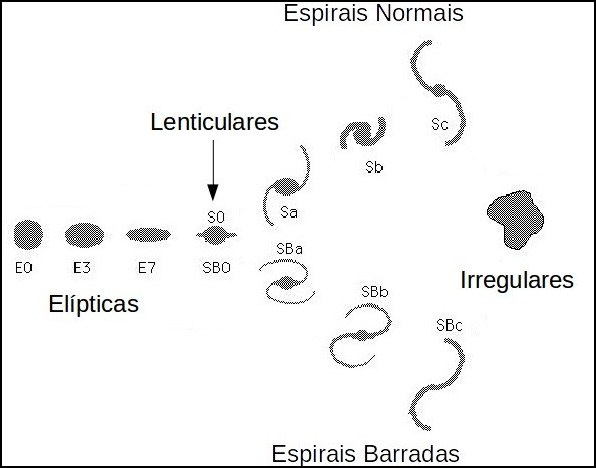
\includegraphics[width=0.6\textwidth]{figuras/espirais_normais.png}
   	\begin{center}
        \normalsize Fonte: \cite{brandt_2017} - modificada \\Classificação morfológica (não evolutiva) das galáxias proposta por Hubble. Trata-se, na verdade, de um primeiro indício de padrão morfológico no Universo próximo.
    \end{center}
	\label{fig:galaxies-classification}
\end{figure}

Galáxias elípticas: são objetos que apresentam isofótas sem nenhuma subestrutura claramente definida. São subdivididas de acordo com o parâmetros n, n = 10(a$-$b)/a, onde 'a' é o semi-eixo aparente maior e 'b' o semi-eixo aparente menor. Existem galáxias elípticas em um grande intervalo de elipticidade ou achatamento aparente ($\epsilon$ = 1$-$b/a), com 0 $\leq$ $\epsilon$ $\leq$ 0.7. Galáxias deste tipo que apresentam achatamento aparente igual a zero apresentam estrutura circular quando projetadas no plano do céu. Um exemplo é a M87 (NGC 4486), cuja cor amarelada representa a predominância de estrelas velhas e frias. De uma maneira geral, quanto maior o valor do parâmetro n, maior o achatamento da estrutura tridimensional da galáxia.

Galáxias S0: são geralmente denominadas de lenticulares e podem ser definidas como uma transição entre as galáxias elípticas e as espirais. Esses objetos apresentam em torno do bojo uma estrutura de disco sem a presença de braços espirais. Um exemplo é a NGC 3115, caracterizada pelo disco e um grande bojo estelar na região central. 

Galáxias espirais: essas objetos apresentam uma estrutura de disco com
braços em formato espiral, e um bojo na região central. Tais galáxias 
apresentam duas subclassificações: espirais normais (S) e espirais barradas (SB). Cada uma dessas subclasses é classificada de acordo com a razão de brilho entre o bojo e o disco, além da quantidade e enrolamento dos braços; assim, de Sa para Sc a razão de brilho entre o bojo e o disco diminui, o número de braços decresce e os braços ficam menos enrolados. NGC 1300 é um exemplo de espiral barrada, com um núcleo central, uma barra, formada por estrelas, gás e poeira, que o atravessa, e braços espirais que se estendem a a partir das extremidades da barra. Por outro lado, temos M31 (galáxia de Andrômedra) como um exemplo de não barrada, a espiral mais próxima da Via Láctea. Se nome é derivado da constelação onde está situada, que, por sua vez, tem seu nome derivado da princesa mitológica Andrômeda. 

Galáxias irregulares: são os objetos que não apresentam uma estrutura em
grande escala bem definida, mas podem exibir várias subestruturas. Como exemplos, podemos destacar a Pequena e a Grande de Magalhães. Representam galáxias anãs e satélites da Via Láctea. A Grande Nuvem é o protótipo de uma subclasse de galáxias irregulares. Estas nuvens foram classificadas por Hubble como Irr I. A Pequena Nuvem é provavelmente um disco distorcido por forças gravitacionais de maré. 

Apesar de comumente aceita, a classificação morfológica não inclui algumas galáxias que apresentam aspectos morfológicos diferenciados destas, ou seja, com características “peculiares\footnote{Peculiaridade do ponto de vista espectroscópico, significa linhas de emissão largas e intensas. Do ponto de vista morfológico, significa características não usuais encontradas nas galáxias presentes no esquema de Hubble, como núcleos deslocados, pontes e caudas de matéria, jatos, anéis, absorções não usuais de poeira, etc.}”, individuais ou em grupos. Tais galáxias também estão presentes no Universo e representam uma rica fonte de informação para o campo da Cosmologia, pois algumas características físicas observadas como a massa, o tamanho e a história de formação estelar, fornecem importantes pistas de como estas intrigantes estruturas se formaram e evoluíram em diferentes redshifts (z).

Do exposto acima, podemos dizer que a classificação morfológica de Hubble se aplica, em uma primeira aproximação, em objetos que não passaram ou não estão passando por intensos processos interativos. Quando uma interação gravitacional encontra-se presente, a morfologia dos objetos envolvidos fica visivelmente afetada, sendo o resultado final observado oriundo de um dos possíveis mecanismos de interação:

\begin{itemize}
\item Colisão: está associado a um parâmetro de impacto no qual os objetos colidem, podendo trocar material ou não; após o evento, os objetos se afastam;

\item Fusão: relaciona-se ao desaparecimento gradativo dos objetos presentes no processo de interação, e ao aparecimento de uma estrutura única, fusionada;

\item Efeito maré: neste caso, um objeto passa próximo de outro(s) e afeta o campo gravitacional, gerando, assim, uma perturbação interna.
\end{itemize}
Nesse sentido, estamos argumentando que o fruto do processo interativo facilita o surgimento de morfologias peculiares. Entretanto, nem toda morfologia irregular é resultado de interação. A natureza intrínseca das galáxias pode ser estudada de forma fotométrica (visual) ou espectroscópica (linhas de absorção/emissão). Portanto, há objetos que podem ter sua morfologia "normal", porém seu espectro ser peculiar com linhas de emissão largas e intensas. A recíproca também é verdadeira para objeto com morfologia peculiar e espectro "normal".

Diante desse contexto contraditório em termos das diferentes características morfológicas observadas, coube ao astrônomo americano Halton Arp (1927-2013) o legado de apresentar e discutir sobre a natureza das galáxias classificadas morfologicamente como peculiares, através do seu \textit{“Atlas of Peculiar Galaxies”}, no qual catalogou e publicou \cite{arp1966atlas} muitas galáxias em processo de interação e de fusão. Na verdade, ele estava preocupado com o fato dos astrônomos de sua época entenderem muito pouco a respeito da evolução das galáxias, de modo que o Atlas tinha o intuito de prover imagens que poderiam fornecer a esses astrônomos dados passíveis de estudos sobre a evolução das mesmas. Mais tarde, Arp usaria seu Atlas como evidência em seu debate sobre os objetos quasi-estelares (quasares), isto é, distante e muito energético, inicialmente descobertos pela emissão em ondas de rádio. Contudo, hoje sabemos que a maioria (90\%) é do tipo “rádio-silencioso” (\textit{radio-quiet}). Também são fontes luminosas no infravermelho, ultravioleta e raios-X, com linhas de emissão largas e intensas. 

Em adição ao trabalho feito para o Hemisfério Norte, um catálogo para o Hemisfério Sul também foi compilado \textit{“A Catalogue of Southern Peculiar Galaxies and Associations”} \cite{arp1987catalogue}, incluindo 25 distintas Categorias\footnote{\url{https://ned.ipac.caltech.edu/level5/SPGA_Atlas/frames.html}} com os mais intrigantes objetos que representam importantes laboratórios para o estudo de vários processos físicos no Universo local (z < 1,0). Halton Arp também é conhecido por ser crítico da teoria do Big Bang e por defender uma Cosmologia não-linear que incorpora um redshift intrínseco. Em particular, os objetos da Categoria 7 ("Galáxias com Jatos") presentes neste último Catálogo foram selecionados para estudo nesta Dissertação de Mestrado, onde discutiremos aspectos individuais (e também comuns) fornecidos pelas técnicas da fotometria e da espectroscopia, além abordar a motivação científica que justificou a nossa escolha de explorar as propriedades nucleares e extranucleares desses objetos.

\section{Por que Estudar as Galáxias com Jatos?}

No catálogo de Arp \& Madore compilado para o Hemisfério Sul, a Categoria 7 trata exclusivamente das galáxias com jatos, cujo entendimento da natureza peculiar pode revelar importantes pistas para a compreensão dos processos físicos que ocorrem na região nuclear desses objetos. Mas, de certa forma, já podemos dizer com uma dada segurança, que determinados processos físicos que levam à determinadas peculiaridades observadas nos objetos que compõem os catálogos de Arp \& Madore (de ambos hemisférios), são, razoavelmente, bem entendidos. Um grande número de objetos são galáxias em processo de interação gravitacional, como, por exemplo, as famosas  galáxias do Redemoinho (M51, Arp 85), e as galáxias Antena (NGC 4038/NGC 4039 ou Arp 244), favorecendo, assim, o conhecimento de determinadas características peculiares. Por outro lado, algumas galáxias anãs presentes são objetos que simplesmente não alcançaram massa suficiente para produzir gravidade que permitisse a formação de uma estrutura mais coesa. NGC 1569 (Arp 210) é um exemplo dessas galáxias anãs. Algumas outras galáxias são caracterizadas como rádio-galáxias. Tais objetos possuem um núcleo galáctico ativo que produzem poderosos jatos relativísticos de gás chamados rádio-jatos (ver Figura \ref{fig:galxy-jet1}). São poderosas fontes de radiação síncrotron, especialmente em ondas de rádio. As rádio-galáxias próximas M87 (Arp 152) e Centaurus A (Arp 153) são alguns desses exemplos.

\begin{figure}[!htb]
	\centering	
    \caption{M87 (NGC 4486, Arp 152). O jato consiste de material gasoso ionizado, elétrons e outras partículas subatômicas, emitidos a uma velocidade próxima da velocidade da luz, a partir do núcleo da galáxia.}
    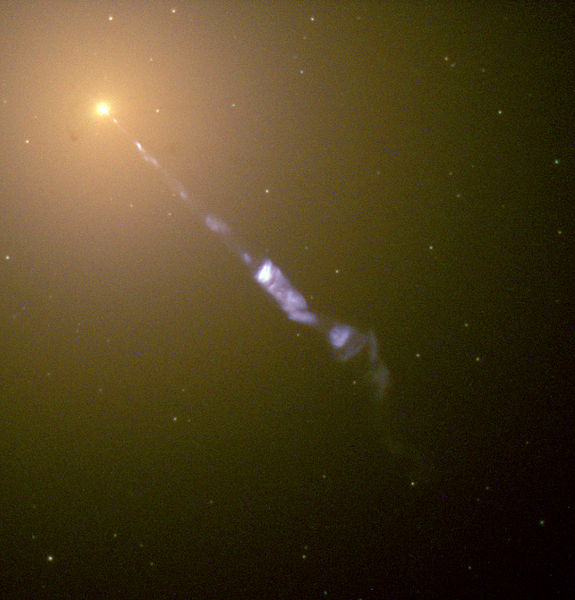
\includegraphics[width=0.6\textwidth]{figuras/m87.jpg}
   	\begin{center}
        \normalsize Fonte: Hubble Space Telescope. \\Observe o jato de partículas que sai da região nuclear de M87 (NGC 4486) e que se estende por cerca de 5 anos-luz.
    \end{center}
	\label{fig:galxy-jet1}
\end{figure}

No caso particular das galáxias com jatos presentes no Categoria 7, trabalhamos com a hipótese de que alguns desses objetos poderiam pertencer, mais adequadamente, à uma outra categoria do catálogo, na qual incluem peculiaridades relacionadas com "caudas", "laços de matéria" e "detritos", ou seja, a Categoria 15: \textit{"Galaxies with Tails, Loops of Material or Debris"}. As Figuras \ref{fig:galaxy-jet2} e \ref{fig:galaxy-jet3} ilustram exemplos destas duas Categorias, evidenciando as peculiaridades em cada caso (jatos e caudas, respectivamente). A partir das Figuras, ficam claras as diferenças entre essas duas peculiaridades. Os jatos são retilíneos, diferentemente das características da Figura 1.4, embora esse assertiva pode ser questionada em alguns objetos. Em ambas imagens, a direção Norte está para cima, e a direção Leste para a esquerda.

\begin{figure}[!htbp]
    \centering
    \caption{Galáxia com Jato. Categoria 7.}
    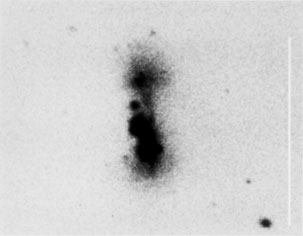
\includegraphics[width=0.7\textwidth]{figuras/2a_am0427-273.png}
   	\begin{center}
    \normalsize Fonte: \cite{arp1987catalogue}.\\AM 0427-273 (Categoria 7) 
    %%Figura 2a.
    \end{center}
    \label{fig:galaxy-jet2}
\end{figure}

\begin{figure}[!htbp]
	\centering	
    \caption{Galáxia com Cauda e Laço de Matéria. Categoria 15.}
    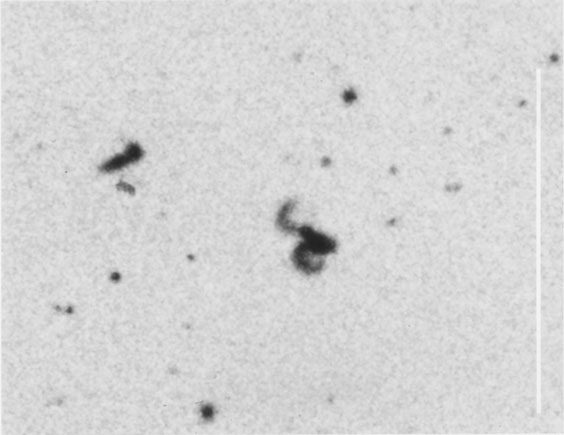
\includegraphics[width=0.7\textwidth]{figuras/2b_AM_0015-315.png}
   	\begin{center}
        \normalsize  Fonte: \cite{arp1987catalogue}.\\AM 0015-315 (Categoria 15)
        %%Figura 2b.
    \end{center}
	\label{fig:galaxy-jet3}
\end{figure}

Na verdade, como se tratam de objetos interagentes, possíveis companheiras acidentalmente superpostas, ou mesmo estrelas projetadas nas imagens, podem dar uma falsa aparência de um jato. Por outro lado, muitos jatos podem ser fracos ou estreitos, também levando a uma falsa impressão. Outros, podem estar centralmente localizados perto dos núcleos de galáxias de alto brilho superficial, onde a análise em diferentes bandas espectrais seriam necessárias para uma correta investigação, visto que as imagens antigas obtidas através de emulsões fotográficas (IIIa-J) poderiam, facilmente, saturar os jatos durante longas exposições.

Nesse sentido, para verificar tais possibilidades e melhor caracterizar a natureza desses objetos, analisamos neste trabalho um conjunto de imagens fotométricas em diferentes bandas: SDSS (B e R, visível), 2MASS (vermelho, J; poeira, K), WISE (infravermelho, 3.4 e 22 $\mu$m), e GALEX (ultravioleta próximo). No entanto, apesar de toda facilidade apresentada, é importante afirmar que nenhuma completude para nossa pesquisa em relação aos jatos interiores deverá ser alcançada nesse trabalho, restando, certamente, outras análises e estudos mais refinados.

As imagens do SDSS dispõem de informação da banda B, que
possibilita uma análise dos componentes de maior energia, e da banda R, componentes mais avermelhados, portanto, de natureza mais fria. Já as imagens do 2MASS e WISE fornecem informações de estrelas velhas e da poeira, que irá depender da banda usada. Com o GALEX, procuramos evidenciar estruturas de altas energias, como estrelas do tipo O e B ou galáxias com núcleos ativos. Usamos a biblioteca "astroquery" do python \cite{sipocz2016astroquery} para fazer o download das imagens, em formato FITS, que é a extensão amplamente usada na Astronomia para imagens e tabelas. A manipulação das imagens foi feita com o astropy.io, pacote do python que acessa aquivos FITS.

Para complementar tais análises, também usamos espectros no óptico observados no Observatório do Pico dos Dias/LNA-MCTIC e extraídos da literatura, 6dF Galaxy Survey (6dFGS), no qual cobrem uma ampla faixa espectral que contêm as principais linhas de absorção e de emissão usadas para investigar algumas propriedades do núcleo, como cinemática, atividade nuclear e população estelar. A Figura \ref{fig:mosaic-spec} ilustra um exemplo dessa compilação espectrofotométrica.

\begin{figure}[!h]
	\centering	
    \caption{Exemplo de análise espectrofotométrica realizada para a galáxia peculiar AM 0007-38 (GALEXASC J000702.28-380300.5). As imagens representam as seguintes bandas, da esquerda para a direita. Superior: DSS2 Blue, 2MASS-J e 2MASS-K. Inferior: WISE 3.4, Wise 2.2 e GALEX FAR UV.}
    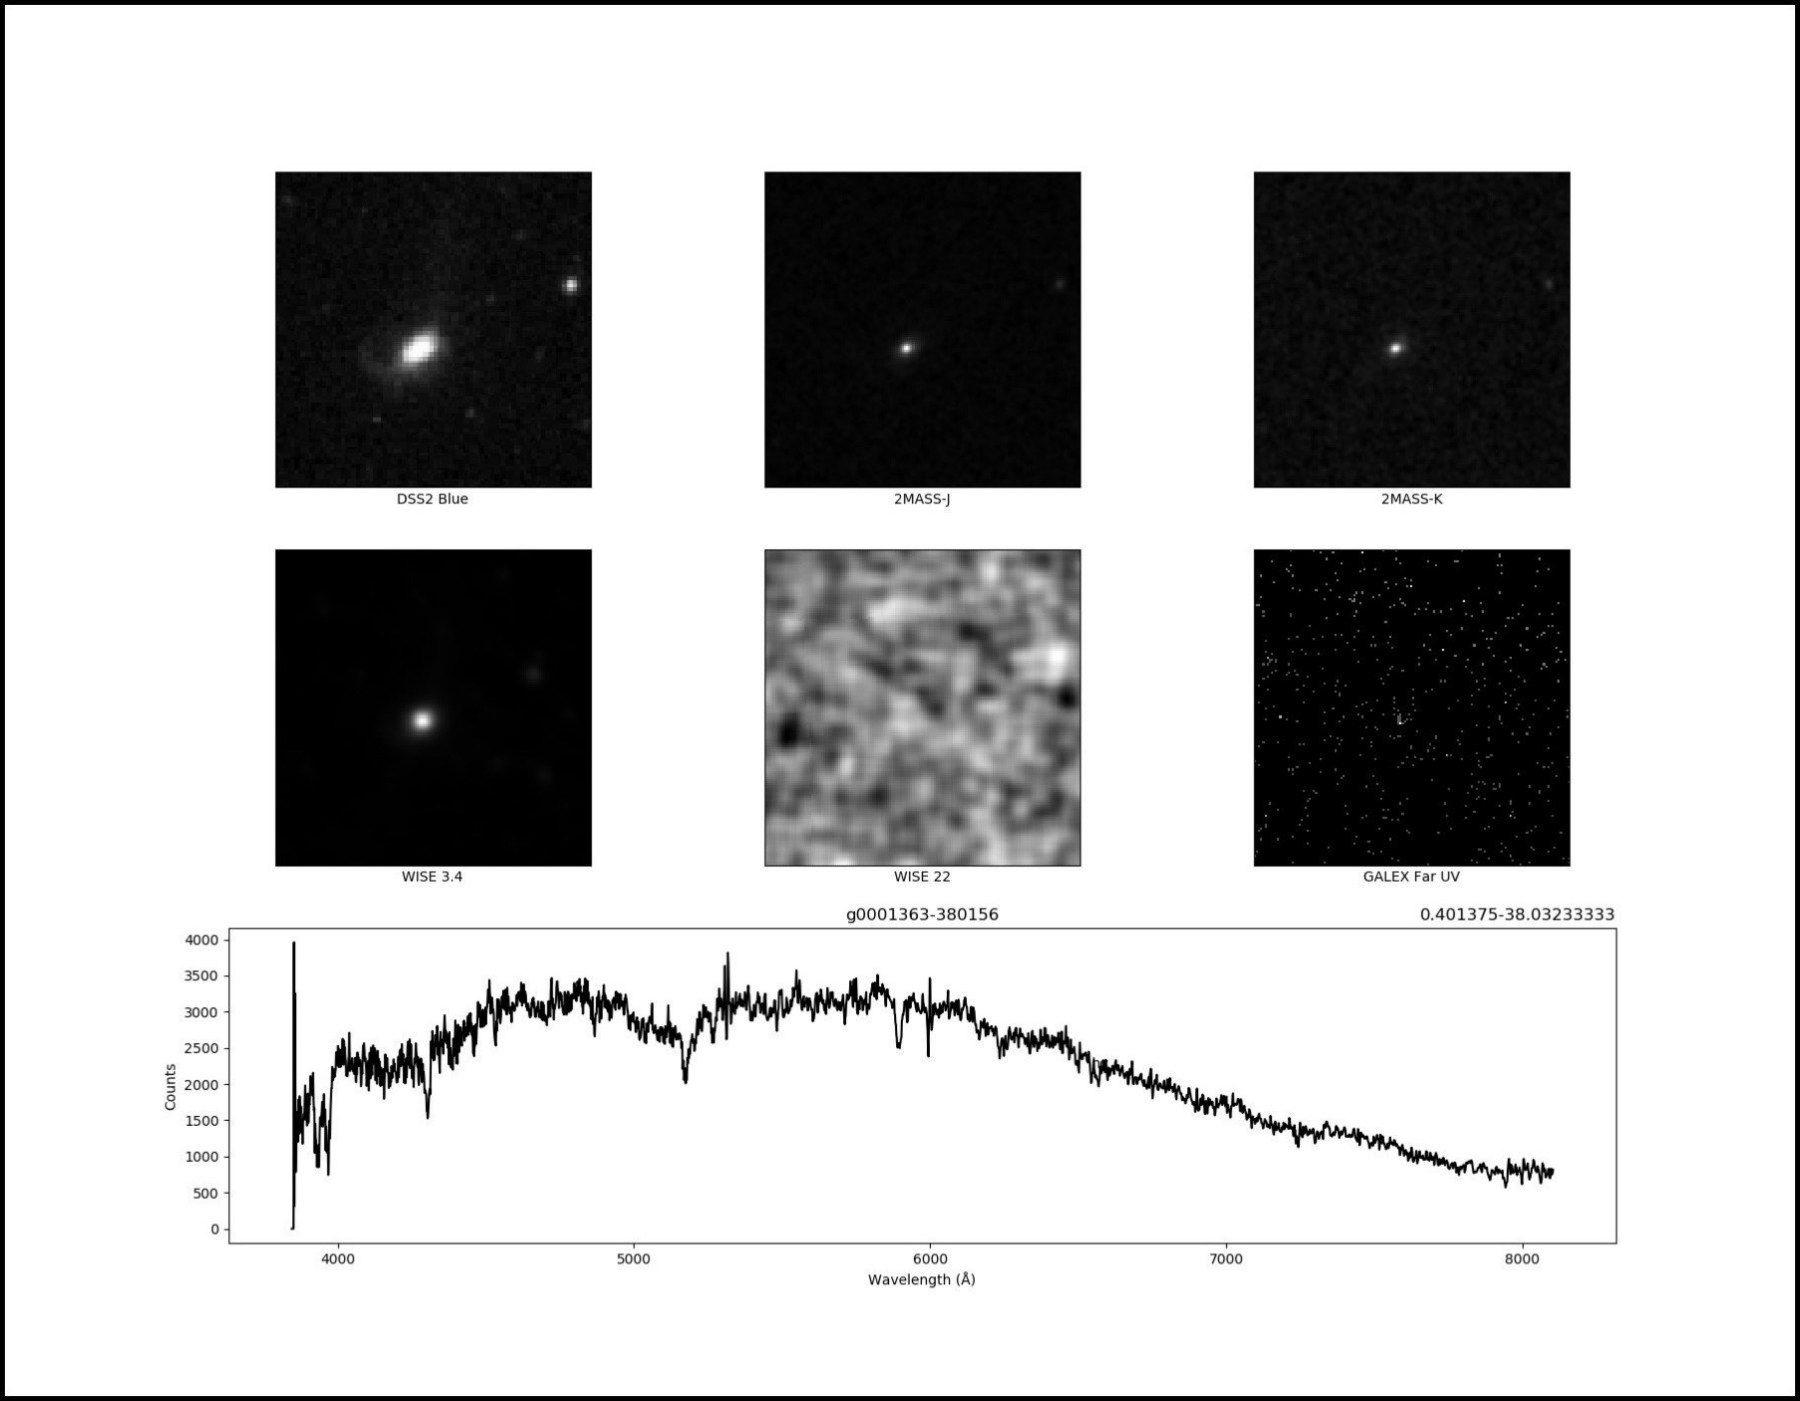
\includegraphics[width=1.0\textwidth]{figuras/fig5.png}
   	\begin{center}
        \normalsize  Fonte: Próprio autor. \\Painel superior: fotometria; Painel inferior: espectroscopia.
        \end{center}
	\label{fig:mosaic-spec}
\end{figure}

\begin{figure}[!htb]
	\centering	
    \caption{Projeção Aitoff}
    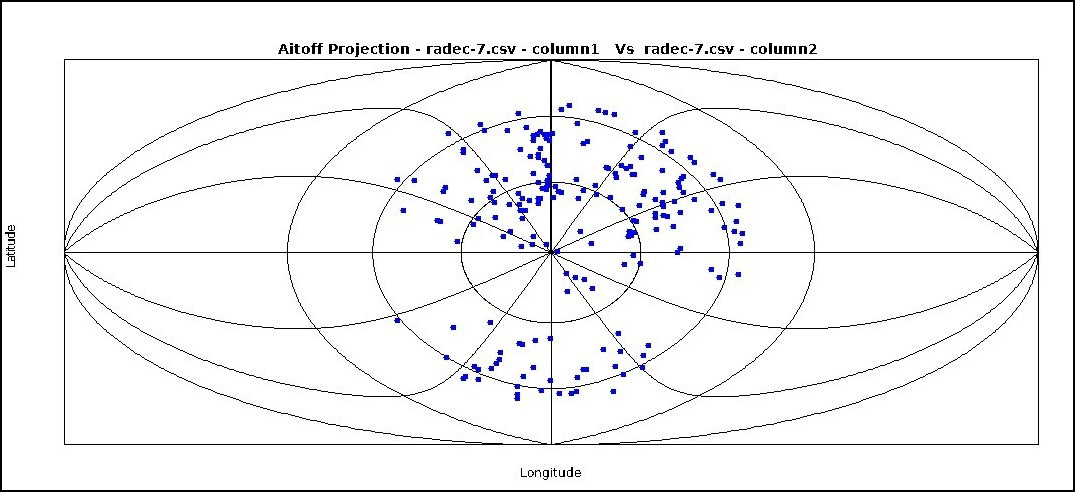
\includegraphics[width=0.8\textwidth]{figuras/southpole.png}
   	\begin{center}
        \normalsize Fonte: Próprio Autor.\\Projeção Aitoff das galáxias presentes na Categoria 7. Visão a partir do pólo sul galáctico.
    \end{center}
	\label{fig:aitoff}
\end{figure}

Ao classificar as galáxias observadas como peculiares na Categoria 7, Arp \& Madore ainda criaram quatro subcategorias para as mesmas: (i) jatos de galáxias centrais elípticas (E) ou do tipo-elíptica (E-like), bastante amplos ou difusos que emergem destes objetos; (ii) jatos de galáxias espirais (ou do tipo espiral), amplos ou estreitos, fracos e difusos, (iii) jatos de vários tipos de galáxias, geralmente um pouco mais estreitos do que nas duas subcategorias precedentes, e que emergem de uma variedade de diferentes tipos de objetos centrais; (iv) jatos de galáxias companheiras, onde filamentos ou jatos emergem de objetos vizinhos, talvez em processos de interação. A Figura \ref{fig:aitoff} ilustra a distribuição (projeção Aitoff) das 125 galáxias com informações espectrais (73 com linhas de emissão) e 52 (com linhas de absorção), de acordo com as coordenadas galácticas.

Do exposto acima, estamos apresentando um rico cenário de investigação científica neste trabalho dissertativo, cujo entendimento ainda não foi completamente estabelecido, embora tenhamos importantes dados na literatura que possam fornecer importantes pistas sobre a natureza desses objetos. Portanto, pretendemos iniciar uma pesquisa que possa direcionar para a compreensão particular desta Categoria. 

\section{Problema Proposto e a Contribuição Científica Associada.}

De um modo geral, as galáxias peculiares conhecidas\footnote{Estudos baseados em surveys (levantamentos astronômicos) poderão classificar e fornecer novas galáxias peculiares. Veja lista em https://en.wikipedia.org/wiki/Astronomical.}, distribuídas em ambos hemisférios, representam uma classe pouco estudada pelas usuais técnicas fotométricas e espectroscópicas (e também polarimétricas), quando comparadas, por exemplo, com as outras galáxias presentes na classificação morfológica de Hubble (ver Figura \ref{fig:galaxies-classification}).

O processo de interação gravitacional envolvendo galáxias no Universo local representa, atualmente, um fenômeno bastante comum e bem documentado. Os diversos tipos morfológicos observados (incluindo nestes as galáxias peculiares) podem ter sua origem, parcial ou total, associado ao fenômeno de interação gravitacional, e não apenas na evolução dinâmica do objeto em um estado físico isolado. Esta propriedade perturbativa e os resultados obtidos sugerem fortemente uma revisão do nosso ponto de vista sobre a classificação e a evolução destes objetos.

A Categoria 7 escolhida para o estudo merece um particular interesse pelo fenômeno físico associado, que é diferente da característica observada em quasares e rádiogaláxias, i.e., a presença de jatos de matéria saindo da fonte central localizada no núcleo destas galáxias. Neste caso, a explicação mais plausível para os jatos nesses objetos (ver Figura \ref{fig:radios}) são as de partículas carregadas movendo-se em um campo magnético (emissão por mecanismo Síncrotron). Como a trajetória seguida pelas partículas é helicoidal, seu movimento é acelerado e elas acabam irradiando energia (ver Figura \ref{fig:radio-eletro}). Portanto, a compreensão da formação dos jatos para o entendimento dos processos físicos nas galáxias peculiares da Categoria 7, representa um problema científico diferente que precisa ser investigado a luz das técnicas espectrofotométricas no óptico, fora, portanto, das usuais observações em rádio e raios-X. Por outro, como interações gravitacionais podem explicar parte desta característica peculiar observada, simulações de n-corpos também representa uma importante fonte de investigação, que poderá ser explorada em um futuro trabalho.

  \begin{figure}[!htb]
	\centering	
    \caption{Jatos e Radiogaláxias.}
    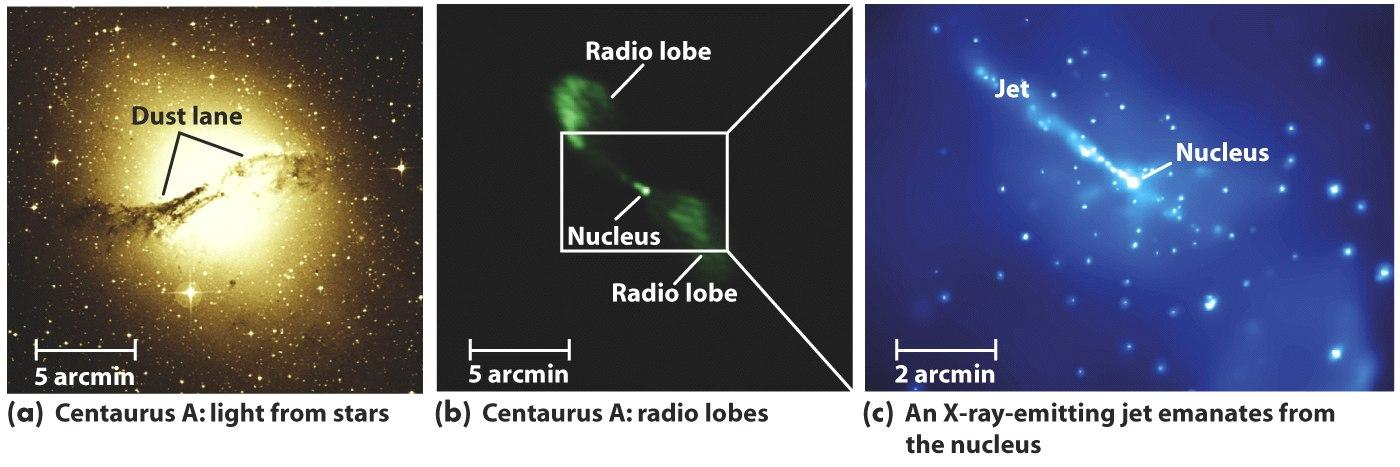
\includegraphics[width=0.9\textwidth]{figuras/radiogalaxia.jpg}
   	\begin{center}
        \normalsize Fonte: \cite{freedman_kaufmann_2008}\\Radiogaláxia Centauro A, uma galáxia elíptica a $\sim$4 Mpc. No visível (imagem da esquerda), a mesma parece como uma elíptica com uma peculiaridade: muita poeira. Em rádio (imagem central) com os lóbulos bem evidentes e em raios-X (direita) um jato saindo do núcleo.   Estes jatos observados em rádio e raios-X indicam processos muito energéticos.
    \end{center}
	\label{fig:radios}
\end{figure}

\begin{figure}[!htb]
	\centering	
    \caption{Radiogaláxias}
    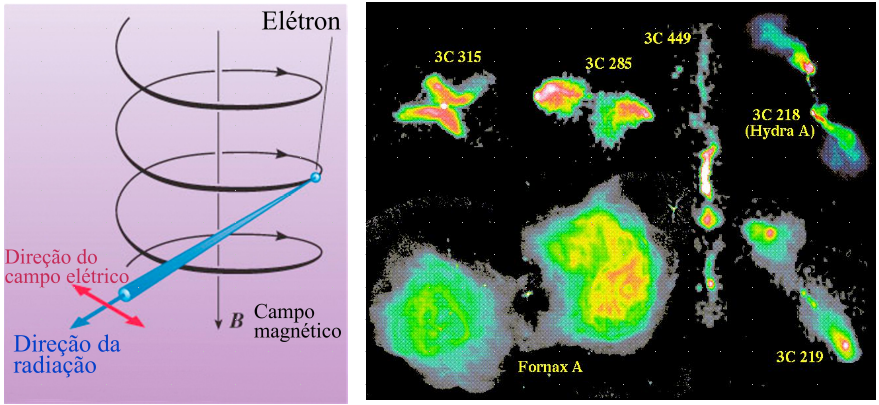
\includegraphics[width=0.9\textwidth]{figuras/radiog_image5.png}
   	\begin{center}
        \normalsize Fonte: \cite{burrows}\\As radiogaláxias estão associadas às galáxias elípticas gigantes. A emissão rádio apresenta diversas morfologias e a fonte de energia está associada ao núcleo.
    \end{center}
	\label{fig:radio-eletro}
\end{figure}

Espectros de galáxias observados em diferentes comprimentos de onda são bastante abundantes e acessíveis em diversos bancos de dados. Alguns surveys extragalácticos são dedicados para a coleta e análise destes espectros, como os projetos SAURON \cite{tim2002sauron}, 6dFGS (JONES et al. 2004), ATLAS 3d \cite{cappellari2011atlas3d}, CALIFA  \cite{sanchez2012califa}, MASSIVE \cite{ma2014massive} e SDSS \cite{alam2015eleventh}. Todos esses projetos apresentam como um de seus objetivos o estudo de populações estelares em galáxias. Porém, boa parte dos mesmos exploram o hemisfério celeste norte, deixando o sul relativamente pouco explorado. Na literatura, existem trabalhos que analisam amostras de espectros de diversas categorias do catálogo de Arp \& Madore, com o objetivo de investigar as propriedades da região central, extranuclear, população estelar, parâmetros físicos e geométricos, etc., por exemplo, \cite{sekiguchi1993spectroscopic,donzelli2000spectroscopic,poppeda2010eso,faundez2015visiting,freitas2017peculiar,krabbe2017interaction}. No entanto, as galáxias selecionadas na Categoria 7 para o presente estudo, são ainda pouco estudadas e muitas delas sem quaisquer informações espectrais detalhadas. Este aspecto assegura, portanto, uma originalidade ao presente trabalho, onde os resultados oriundos da síntese espectral via código STARLIGHT \cite{cid2004star,fernandes2005semi,asari2007history} (inéditos para a quase totalidade) e das análises em diagramas de diagnóstico a partir do espectro residual obtido através da síntese, permitirão contribuir para um melhor conhecimento desses objetos peculiares e, sobretudo, da natureza dos jatos observados na banda óptica.


 %%%%%%%%%%%%%%%%%%%%%%%%%%%%%%%%%%%%%%%%%%%%%%%%%%%%%%%%%%%%%%%%%%%%%%%%%%%%%%%%%%%%%%%%%%%%%%%%
 


%%%%%%%%%%%%%%%%%%

